\section*{Problema 05}

\textbf{Show that the function $f (x) = 8x_1 + 12x_2 + x^2_1 - 2x_2^2$ has only one stationary point, and that it is neither a maximum or minimum, but a saddle point. Plot the contour lines of f.}

Calculando la primer derivada parcial con respecto a $x_1$ de la función $f(x)$ se obtiene lo siguiente:

\begin{equation*}
    \dpartial{f(x)}{x_1} = 8+2x_1
\end{equation*}

Calculando la primer derivada parcial con respecto a $x_2$ de la función $f(x)$ se obtiene lo siguiente:

\begin{equation*}
    \dpartial{f(x)}{x_2} = 12-4x_2
\end{equation*}

Por lo tanto, el punto crítico obtenido es $x_c=(-4,3)$.

Calculando el hessiano de $f(x)$ se obtiene lo siguiente:

\begin{align*}
    \nabla^2 f(x)   & = \begin{vmatrix}
        \dpartial{^2f(x)}{x_1^2}           & \dpartial{^2f(x)}{x_1\partial x_2} \\
        \dpartial{^2f(x)}{x_2\partial x_1} & \dpartial{^2f(x)}{x_2^2}
    \end{vmatrix} = \begin{vmatrix}
        2 & 0  \\
        0 & -4
    \end{vmatrix} \\
    |\nabla^2 f(x)| & = -8
\end{align*}

Como $\nabla^2 f(x)<0$ para cualquier x, entonces $x_c$ es un punto silla.

En la figura \ref{fig:problem_5} se representan las curvas de nivel de la función $f(x)$.

\begin{figure}[H]
    \centering
    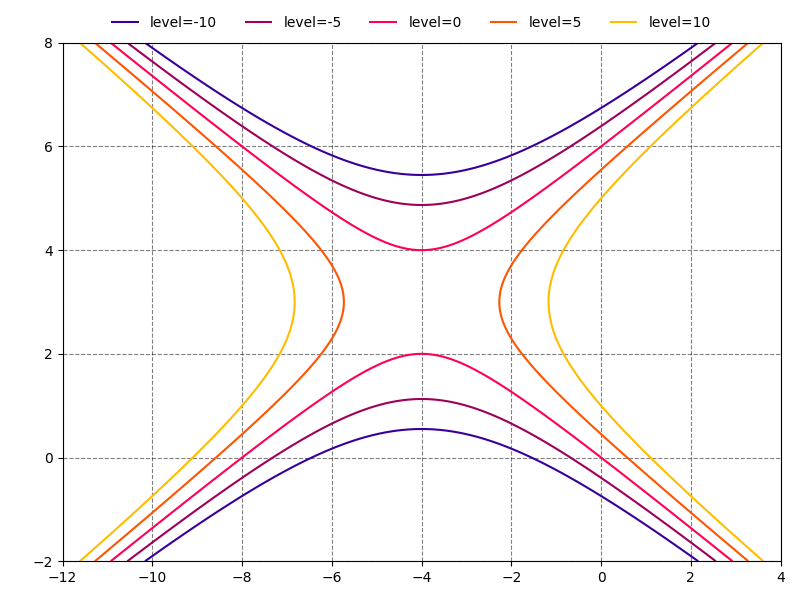
\includegraphics[width=12cm]{Graphics/problem05.png}
    \caption{Curvas de niel de la función $f(x)$.}
    \label{fig:problem_5}
\end{figure}